\documentclass[10pt]{article}

\pagestyle{empty}

\setlength{\textheight}{250mm}
\setlength{\textwidth}{180mm}
\setlength{\oddsidemargin}{-8mm}
\setlength{\topmargin}{-1.5cm}

\usepackage{amsmath}
\usepackage{amsthm}
\usepackage{psfrag}
\usepackage{graphicx}
\usepackage{bm}
\usepackage{mathrsfs}
\usepackage{icomma} % pacchetto per limitare lo spazio standard posto dopo la virgola in caso che la virgola sia tra cifre
\usepackage{amsfonts} % amplia i caratteri matematici disponibili
\usepackage{amssymb}
%\usepackage{wrapfig}
\usepackage{empheq}

\usepackage{epstopdf}
\usepackage[utf8x]{inputenc}
\usepackage{ifthen}

\usepackage{caption}

\usepackage[italian]{babel}
%\usepackage[latin1]{inputenc}

\usepackage{subfig}

\usepackage{pgfplots}
\pgfplotsset{compat=1.9}

%\input{def}

%\newcommand{\kg}{\textrm{kg}}
%\newcommand{\K}{\textrm{K}}
%\newcommand{\m} {\textrm{m}}
%\newcommand{\dm}{\textrm{dm}}
%\newcommand{\cm}{\textrm{cm}}
%\newcommand{\mm}{\textrm{mm}}
%\newcommand{\s} {\textrm{s}}
%\newcommand{\N} {\textrm{N}}
%\renewcommand{\Pa}{\textrm{Pa}}

\def \flagSect{0} % 1    : numerazione
		  % else : niente
%\newcommand{\taitol}[1]  % stile titolo
%{
%%{\textit{#1}}
%{#1}
%}
\def \soluzione{Soluzione}
\def \partePrima{Concetti. }
\def \parteSeconda{Svolgimento. }
%\def \parteTerza{}
\newcommand{\sol}{\subsubsection*{\soluzione}}
\newcommand{\partone}{\ \ \ \ \ \textbf{\partePrima}}
\newcommand{\parttwo}{\vspace{0.2cm}\textbf{\parteSeconda}}

\ifnum\flagSect=1
\newtheorem{esercizio}{Esercizio}%[section]
\else
\newtheorem*{esercizio}{Esercizio}
\fi

\newtheorem*{teorema}{Teorema}
\newtheorem*{lemma}{Lemma}

% ###########################################################
%\def \flagSect{0} % 1    : numerazione
		  % else : niente
%\newcommand{\taitol}[1]  % stile titolo
%{
%%{\textit{#1}}
%{#1}
%}
\def \soluzione{Soluzione}
\def \partePrima{Concetti. }
\def \parteSeconda{Svolgimento. }
%\def \parteTerza{}
\newcommand{\sol}{\subsubsection*{\soluzione}}
\newcommand{\partone}{\ \ \ \ \ \textbf{\partePrima}}
\newcommand{\parttwo}{\vspace{0.2cm}\textbf{\parteSeconda}}

\ifnum\flagSect=1
\newtheorem{esercizio}{Esercizio}%[section]
\else
\newtheorem*{esercizio}{Esercizio}
\fi

\newtheorem*{teorema}{Teorema}
\newtheorem*{lemma}{Lemma}

% ###########################################################
%\def \flagSect{0} % 1    : numerazione
		  % else : niente
%\newcommand{\taitol}[1]  % stile titolo
%{
%%{\textit{#1}}
%{#1}
%}
\def \soluzione{Soluzione}
\def \partePrima{Concetti. }
\def \parteSeconda{Svolgimento. }
%\def \parteTerza{}
\newcommand{\sol}{\subsubsection*{\soluzione}}
\newcommand{\partone}{\ \ \ \ \ \textbf{\partePrima}}
\newcommand{\parttwo}{\vspace{0.2cm}\textbf{\parteSeconda}}

\ifnum\flagSect=1
\newtheorem{esercizio}{Esercizio}%[section]
\else
\newtheorem*{esercizio}{Esercizio}
\fi

\newtheorem*{teorema}{Teorema}
\newtheorem*{lemma}{Lemma}

% ###########################################################
%\input{logicNumb}
%\newcommand{\sectionIf}[2]
%{
%   \ifthenelse{\equal{#1}{1}}
%              {\subsection{#2}}{\subsection*{#2}}
%}
% ###########################################################

%\newcommand{\sectionIf}[2]
%{
%   \ifthenelse{\equal{#1}{1}}
%              {\subsection{#2}}{\subsection*{#2}}
%}
% ###########################################################

%\newcommand{\sectionIf}[2]
%{
%   \ifthenelse{\equal{#1}{1}}
%              {\subsection{#2}}{\subsection*{#2}}
%}
% ###########################################################


\begin{document}

\begin{center}
\textbf{Esercizi per il corso di Fluidodinamica} 
\medskip
\end{center}


\noindent
\begin{tabular}{cc}
\begin{minipage}{0.60\textwidth}
\begin{exerciseS}[Corrente di Taylor-Couette]
Si consideri la corrente piana fra due cilindri coassiali rotanti.
Si misura la velocit\`a in due punti posti rispettivamente a $1/4$ e 
$3/4$ del gap fra i due cilindri: 
$u_{\theta,1/4} = 0.5\ m/s$, 
$u_{\theta,3/4} = 0.8\ m/s$.
Si determini la velocit\`a di rotazione dei due cilindri nonch\'e
la pressione in corrispondenza del cilindro interno sapendo che
la pressione in corrispondenza del cilindro esterno vale $5\ Pa$,
che la densit\`a del fluido \`e pari a $1.225\ kg/m^3$,
che il diametro del cilindro interno \`e $d =2 R_1=0.1 \ m$ e che il diametro 
del cilindro esterno \`e $D = 2 R_2 = 0.16 \ m$.
 
($\Omega_{1}=6.663\ s^{-1}$, $\Omega_{2}=11.743\ s^{-1}$ \newline
$P(r) = P_2 - \rho \left[ \dfrac{1}{2} A^2 (R_2^2 - r^2) + 2 A B ln \dfrac{R_2}{r} - 
      \dfrac{1}{2}B^2 \left( \dfrac{1}{R^2} - \dfrac{1}{r^2} \right)  \right]$, \newline
      con $u_{\theta}(r) = A r + B/r$\ .
 )
\end{exerciseS}
\end{minipage}
&
\begin{minipage}{0.35\textwidth}
   \begin{center}
   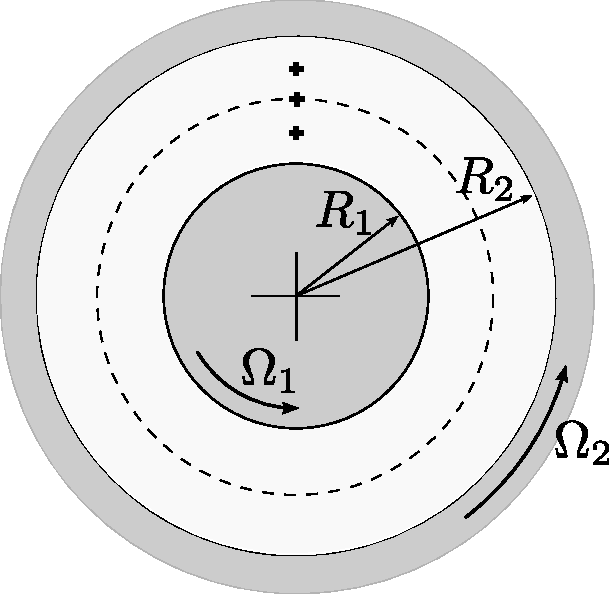
\includegraphics[width=0.90\textwidth]{./fig/slnEsatte-taylor-couette-2}
   \end{center}
\end{minipage}
\end{tabular}

\sol

\partone Soluzione esatte delle equazioni di Navier-Stokes in geometria cilindrica. Corrente di Taylor-Couette.

\begin{equation}
  \begin{cases}
    \rho \dfrac{\partial u_r}{\partial t}
    + \rho \left( \bm{u} \cdot \bm{\nabla}u_r - \dfrac{u_\theta^2}{r} \right)
    - \mu \left(\nabla^2 u_r 
       - \dfrac{u_r}{r^2} 
       - \dfrac{2}{r^2}\dfrac{\partial u_\theta}{\partial \theta} \right)  
       + \dfrac{\partial p}{\partial r} = f_r \\
    \rho \dfrac{\partial u_\theta}{\partial t}
    + \rho \left( \bm{u} \cdot \bm{\nabla} u_\theta + \dfrac{u_\theta u_r}{r} \right)
    - \mu \left(\nabla^2 u_\theta 
       - \dfrac{u_\theta}{r^2} 
       + \frac{2}{r^2}\dfrac{\partial u_r}{\partial \theta}  \right) 
    + \dfrac{1}{r} \frac{\partial p}{\partial \theta} = f_\theta\\
    \rho \dfrac{\partial u_z}{\partial t}
    + \rho \bm{u} \cdot \bm{\nabla} u_z
    - \mu \nabla^2 u_z
    + \dfrac{\partial p}{\partial z} = f_z \\ \\
    \dfrac{1}{r}\dfrac{\partial}{\partial r}\left( r u_r \right) 
    + \dfrac{1}{r}\dfrac{\partial u_\theta}{\partial \theta} 
    + \dfrac{\partial u_z}{\partial z} = 0
  \end{cases}
  \end{equation}
  con 
  \begin{equation}
  \begin{aligned}
  & \bm{a} \cdot \bm{\nabla} b = a_r \dfrac{\partial b}{\partial r} 
     + \dfrac{a_\theta}{r} \dfrac{\partial b}{\partial \theta}  
     + a_z \dfrac{\partial b}{\partial z} \\
  & \nabla^2 f = \dfrac{1}{r}\dfrac{\partial}{\partial r}
                      \left(r \frac{\partial f}{\partial r} \right) +
               \frac{1}{r^2} \frac{\partial^2 f}{\partial \theta^2} + 
               \frac{\partial^2 f}{\partial z^2} 
  \end{aligned}
  \end{equation}

\parttwo Il problema viene risolto calcolando prima le velocità angolari dei cilindri e
successivamente la pressione.

\begin{itemize}

\item La soluzione di Taylor-Couette viene ricavata dall'espressione semplificata delle equazioni di Navier-Stokes,
\begin{equation}
\begin{cases}
  -\rho \dfrac{u^2_\theta}{r} + \dfrac{\partial P}{\partial r} = 0 \\
  -\dfrac{1}{r}\dfrac{\partial}{\partial r} \left( r \dfrac{\partial u_\theta}{\partial r}  \right)  + \dfrac{u_\theta}{r^2}= 0 \ ,
\end{cases}
\end{equation}
ottenute imponendo che il campo di moto sia bidimensionale $\bm{u}(\bm{r}) = u_{\theta}(r,\theta) \bm{\hat{\theta}} + u_r (r,\theta) \bm{\hat{r}}$, che la soluzione sia omogenea rispetto alla coordinata $\theta$ e sfruttando le condizioni al contorno e il vincolo di incomprimibilità per ricavare $u_r(\theta) = 0$.
%
Sia il campo di pressione sia il campo di velocità dipendono solamente dalla coordinata radiale, $P = P(r)$, $u_\theta = u_\theta (r)$. Le derivate parziali possono essere quindi trasformate in derivate ordinarie. La seconda equazione è disaccoppiata dalla prima e può essere risolta, una volta imposte le condizioni al contorno. Trovato il campo di moto da questa equazione, la prima viene usata per calcolare il campo di pressione. La seconda equazione può essere riscritta come (svolgere le derivate per credere!)
\begin{equation}
\begin{cases}
  -\left(\dfrac{1}{r} \left(r u_\theta\right)'\right)' = 0 \\
  u_\theta(R_1) = \Omega_1 R_1 \\
  u_\theta(R_2) = \Omega_2 R_2 \\
\end{cases}
\Rightarrow
\begin{cases}
  u_\theta(r) = A r + \dfrac{B}{r} \ \ \ \text{A,B from b.c.} \\
  u_\theta(R_1) = \Omega_1 R_1 \\
  u_\theta(R_2) = \Omega_2 R_2 \\
\end{cases}
\end{equation}
%
Il campo di moto tra due cilindri coassiali rotanti è
\begin{equation}
  u_\theta(r) = \frac{\Omega_2 R_2^2 - \Omega_1 R_1^2}{R_2^2-R_1^2} r +
   \frac{(\Omega_1 - \Omega_2)R_1^2 R_2^2}{R_2^2-R_1^2}\frac{1}{r} \ .
\end{equation}
%
\begin{remark} La soluzione esatta di Taylor-Couette è facile da ricavare, se si ricorda
che è la somma di una rotazione rigida e un vortice irrotazionale: imponendo la forma
$u_\theta (r) = A r + B/r$ e le condizioni al contorno,
\begin{equation}
 u_{\theta}(R_1) = \Omega_1 R_1 \qquad , \qquad  u_{\theta}(R_2) = \Omega_2 R_2
\end{equation}
si ottiene la formula voluta.
\end{remark}

\item Calcolo delle velocità angolari dei cilindri. Nota la forma del campo di moto e
le velocità in due punti a diversi raggi, è possibile calcolare $\Omega_1$, $\Omega_2$
 risolvendo un sistema lineare di due equazioni nelle due incognite.
%
Note le misure di velocità $u_{\theta,1/4} = u_{\theta}(r_{1/4})$, $u_{\theta,3/4} = u_{\theta}(r_{3/4})$, il sistema risolvente diventa:
\begin{equation}
 \displaystyle\begin{bmatrix}
  -\frac{R_1^2}{R_2^2-R_1^2}r_{1/4} + \frac{R_1^2 R_2^2}{R_2^2-R_1^2}\frac{1}{r_{1/4}} & \quad
   \frac{R_2^2}{R_2^2-R_1^2}r_{1/4} - \frac{R_1^2 R_2^2}{R_2^2-R_1^2}\frac{1}{r_{1/4}} \\ 
  -\frac{R_1^2}{R_2^2-R_1^2}r_{3/4} + \frac{R_1^2 R_2^2}{R_2^2-R_1^2}\frac{1}{r_{3/4}} & \quad
   \frac{R_2^2}{R_2^2-R_1^2}r_{3/4} - \frac{R_1^2 R_2^2}{R_2^2-R_1^2}\frac{1}{r_{3/4}} \\
 \end{bmatrix}
 \displaystyle\begin{bmatrix}
  \Omega_1 \\ \Omega_2
 \end{bmatrix} =
 \displaystyle\begin{bmatrix}
  u_{\theta,1/4} \\ u_{\theta,3/4}
 \end{bmatrix}
\end{equation}

%La soluzione di Taylor-Couette può essere ricavata abbastanza facilmente semplificando le  equazioni di Navier-Stokes scritte in coordinate cilindriche, dopo aver fatto le opportune ipotesi (quali?). Le componenti in direzione radiale e tangenziale dell'equazione della quantità di moto diventano:

\item Calcolo della pressione. Una volta noto il campo di moto, è possibile calcolare il campo di pressione dalla componente radiale dell'equazione della quantità di moto,
\begin{equation}
\begin{aligned}
  P'(r) & = \rho \dfrac{u_\theta^2}{r} \quad , \quad \text{con $P(R_2) = P_2$} \\
 & \quad \rightarrow \quad
 \int_{r}^{R_2} \dfrac{dP}{dr} dr 
      = \int_r^{R_2} \rho \dfrac{1}{r} \left( A r + \dfrac{B}{r} \right)^2 dr
\end{aligned}
\end{equation}
%
Da questa si ricava
\begin{equation}
  P(r) = P_2 - \rho \left[ \dfrac{1}{2} A^2 (R_2^2 - r^2) + 2 A B ln \dfrac{R_2}{r} - 
      \dfrac{1}{2}B^2 \left( \dfrac{1}{R^2} - \dfrac{1}{r^2} \right)  \right] \ .
\end{equation}


\end{itemize}


%%%%%%%%%%%%%%%%%%%%%%%%%%%%%%%%%%%%%%%%%%%%%%%%%%%%%%%%%%%%%%%%%%

%%%%%%%%%%%%%%%%%%%%%%%%%%%%%%%%%%%%%%%%%%%%%%%%%%%%%%%%%%%%%%%%%%

%%%%%%%%%%%%%%%%%%%%%%%%%%%%%%%%%%%%%%%%%%%%%%%%%%%%%%%%%%%%%%%%%%


%%%%%%%%%%%%%%%%%%%%%%%%%%%%%%%%%%%%%%%%%%%%%%%%%%%%%%%%%%%%%%%%%%

%%%%%%%%%%%%%%%%%%%%%%%%%%%%%%%%%%%%%%%%%%%%%%%%%%%%%%%%%%%%%%%%%%
%%%%%%%%%%%%%%%%%%%%%%%%%%%%%%%%%%%%%%%%%%%%%%%%%%%%%%%%%%%%%%%%%%

\end{document}
